%
% hardware.tex
%
% Copyright (C) 2020 by SpaceLab.
%
% Flatsat Platform Documentation
%
% This work is licensed under the Creative Commons Attribution-ShareAlike 4.0
% International License. To view a copy of this license,
% visit http://creativecommons.org/licenses/by-sa/4.0/.
%

%
% \brief Hardware chapter.
%
% \author Gabriel Mariano Marcelino <gabriel.mm8@gmail.com>
%
% \institution Universidade Federal de Santa Catarina (UFSC)
%
% \version 0.1.0
%
% \date 2020/10/11
%

\chapter{Hardware} \label{ch:hardware}

\section{Antenna Interfaces}

\subsection{Impedance Control of the RF Tracks}

\begin{figure}[!ht]
    \begin{center}
        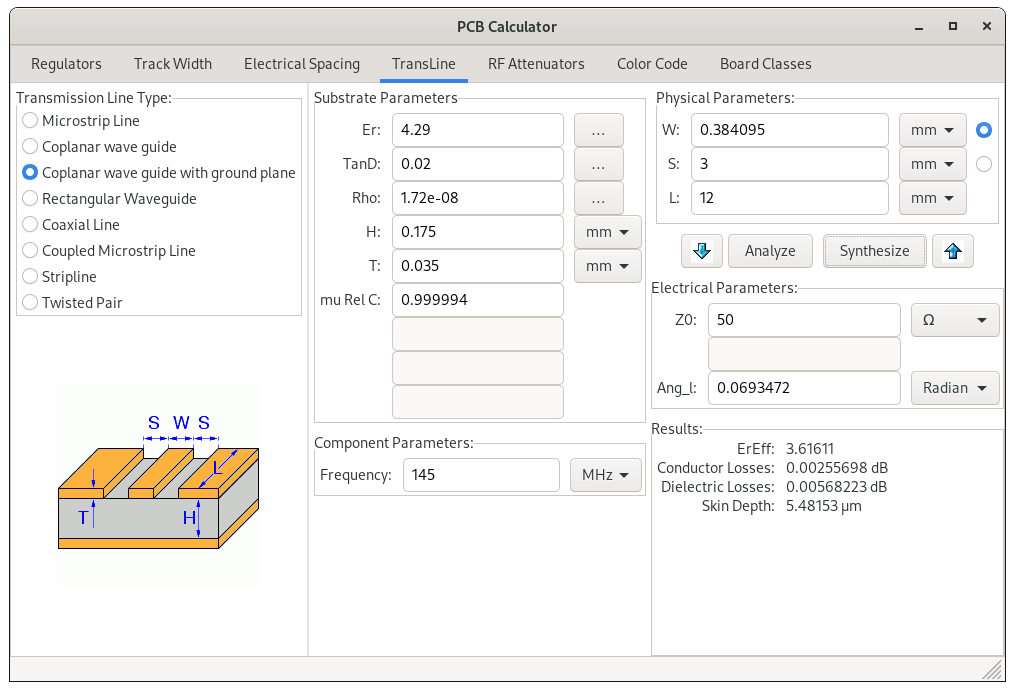
\includegraphics[width=\textwidth]{figures/rf-track-width}
        \label{fig:rf-track-width-calc}
        \caption{Calculation of the width of the RF tracks.}
    \end{center}
\end{figure}

\begin{figure}[!ht]
    \begin{center}
        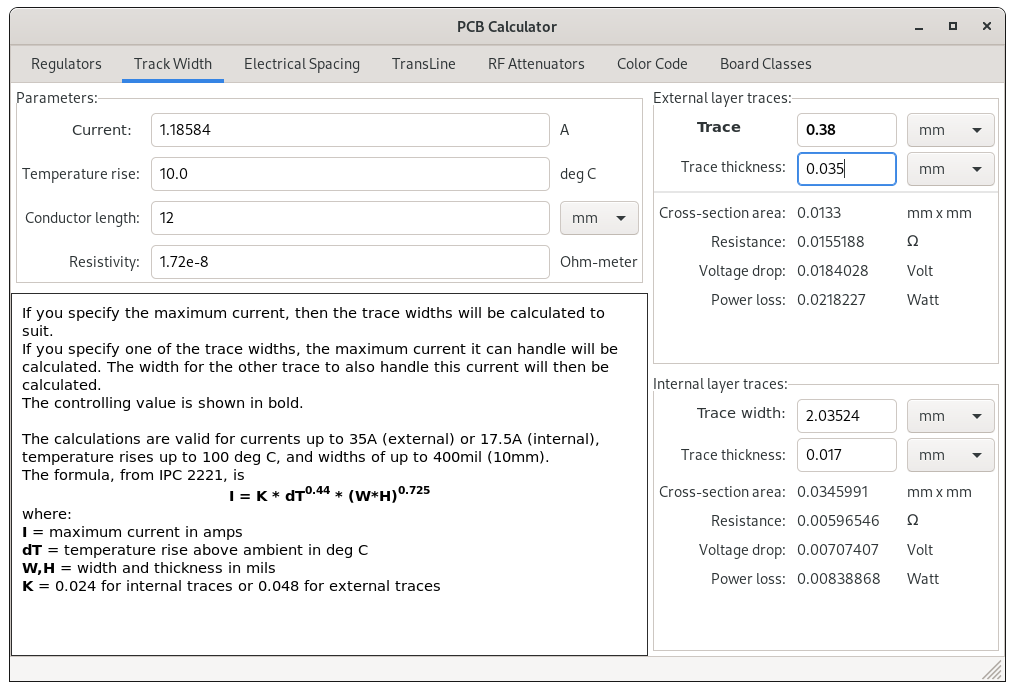
\includegraphics[width=\textwidth]{figures/rf-track-width-power}
        \label{fig:rf-track-width-power-calc}
        \caption{Power dissipation of the RF tracks.}
    \end{center}
\end{figure}
